\begin{figure}[h]
\begin{center}
  \subfloat[]{
    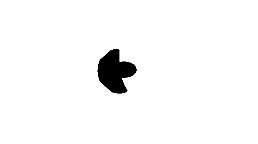
\includegraphics[width=0.2\textwidth]{imgs/segmentationnormal75.png}
    \label{fig:segmentation75}
  }
  \subfloat[]{
    
\includegraphics[width=0.2\textwidth]{imgs/segmentationnormal150.png}
    \label{fig:segmentation150}
  }
  \subfloat[]{
    
\includegraphics[width=0.2\textwidth]{imgs/segmentationnormal225.png}
    \label{fig:segmentation225}
  }
  \subfloat[]{
    
\includegraphics[width=0.2\textwidth]{imgs/segmentationnormal250.png}
    \label{fig:segmentation250}
  }
  \subfloat[]{
    
\includegraphics[width=0.2\textwidth]{imgs/segmentationnormal275.png}
    \label{fig:segmentation275}
  }
\end{center}
\caption{A segmentation method in progress showing the segmentation at
  iteration 75, 150, 225, 250 and 275.}
\label{fig:segmentation}
\end{figure}


Segmentation is an incredibly important area of interest when it comes
to Medical Imaging. Segmentation is the problem of partitioning a
digital image into multiple segments that are more meaningful and
easier to analyse. Typically one would like to locate the boundaries
in a picture such as lines, curves, etc.

The result of a segmentation is a set of segments that covers the
entire picture. All pixels in each segment shares properties based one
how the picture is segmented. It could be color or intensity. Adjecent
regions are significantly different based on these characteristics.

A technique is to initially start inside the object you want to
segment and then expand it like a balloon until the surface reaches
the edge of the contour.

To illustrate segmentation in a level set model, I have implemented
two different algorithms which are described in sections
\vref{segmentation:sec:algorithm1} and
\vref{segmentation:sec:algorithm2}.


\section{Implicit vs. Explicit representation}


Since segmentation techniques normally are used to locate organs in MR
scans or measure the volume of tissue, eg. from real people, it is
very important that the segmentation is correct and that it is
fast. Therefore, we have to convince ourselves that our technique can
find the contour in images even though they can contain a lot of noise
and artefacts.

In an explicit representation, we have the problem that when we only
represent the surface, we run into trouble when segmenting artefacts
as can be seen in figure \vref{segmentation:fig:explicit}. The problem
is that the segmentation can not figure out to skip over the artefacts
which resolves in a segmentation that never terminates. There exist
algorithms that try to skip the artefacts, but they are prone to
failure.

% \image{image, scale, caption, label}
\image{explicit.png}{0.3}{We see how the segmentation, using an
  explicit representation has trouble with artefacts in the
  picture. The surface is about to wrap around it self creating an
  endless loop around the artefact.}{segmentation:fig:explicit}

In an implicit representation, the problem vanishes since we look at
the larger picture and not just the boundary of the current
segmentation. Because we use a level set to solve the problem, when
our algorithm reaches an artefact the solver simply goes around it and
merge at the other side.


\section{Algorithm 1 - Moving in the normal direction}
\label{segmentation:sec:algorithm1}

\begin{comment}
Start med noget mere overordnet og gå derefter i detaljer.

Læs igennem så det ikke står spredt men samlet.

Indsæt afsnit hvor jeg går direkte i dybden og overvej at fjerne
ligning 1.1

\end{comment}

In this algorithm I have been inspired by the balloon algorithm from
\cit{bowden1997real}.  To segment a part of an image, we start with a
small area inside the area we want to segment and grow it in the
normal direction if we have not reached the boundary yet. We know if
we have hit the boundary if the value of the pixel is smaller/larger
than a specified treshold we define. If we have crossed the border
(again based on the threshold value), we shrink that point of the
surface by going in the reverse direction of the normal.

% \image{image, scale, caption, label}
\image{normalDirection.png}{0.3}{In the figure, we see how the
  segmentation grows in the normal
  direction}{segmentation:fig:normaldirection}


Basically we solve the following equation:

\begin{equation}
  \phi_{t} + a|\nabla{\phi}| = 0
\end{equation}

which is easily achieved using the code below: 

\begin{listing}
\begin{lstlisting}[language=c++]
for(unsigned int x=0; x<width; x++) {
    for(unsigned int y=0; y<height; y++) {
        [...]
        if (picture(x,y) > threshold) {
            phi(x,y) += a;
            growth += -a;
        } else {
            phi(x,y) += -a;
            growth += a;
        }
    }
}
[...]

if (growth / ``number of pixels moving'' < tTreshold) {
    done = true;
}
\end{lstlisting}
\label{segmentation:code}
\end{listing}


We want to be able to terminate the segmentation when we have found
the correct area. We do this by looking at the zero iso-surface and
check how much the surface is moving. When it slows down we know that
we have found the area we want to segment.

This is a quite simple algorithm which surprisingly produces good
results. On a picture of dimensions 512 x 512 it stops after
approximately 250-300 iterations which is quite good. We could do this
many times faster if we choose to implement the reinitialization step
on the GPU via CUDA.

In order to make the segmentation algorithm stop when it reaches the
boundary, we calculate the following factor:

\begin{equation*}
 \textrm{factor} = \textrm{growth } / \textrm{ number of pixels moving on iso-surface}
\end{equation*}

Which is a number that goes towards zero when the iso surface stops
moving. To see this, think about what happens when we have reached the
boundary. since about half of the iso-surface is increased and the
other half is going to be decreased the factor should be approximately
zero. \texttt{tThreshold} is set to 0.03 through experiments.



\section{Algortihm 2 - Edge detection}
\label{segmentation:sec:algorithm2}

% \image{image, scale, caption, label}
\image{advsegmentation.png}{0.7}{We see the result of computing the
  final image in the preprocessing step where the algorithm calculates
  the edges. On the left, we see the original picture we want to
  segment. On the right, the final image we use in the segmentation
  algorithm is showed. The final picture is generated by spotting zero
  crossings and by that creating a picture containing the edge
  information we need. }{segmentation:fig:advancedsegmentation}

Algorithm 2 is more advanced and tries to find the edges beforehand to
increase the likelyhood that we segment the correct part, see
\cit{museth2002level}. It builds a series of images and solves the
following equation:

\begin{equation}
\label{segmentation:equation:advanced}
  \dfrac{\partial \phi}{\partial t} - \textrm{grad}(D) \cdot \textrm{grad}(\phi) = 0
\end{equation}
t
where image D has the edge information with an edge denoted as a one and a nonedge as a zero.

To compute image D we have to go through a number of steps. First, we
compute an image A where every pixel is the norm of the gradient in
the original image. Secondly, we compute an image B where every pixel
is the gradient in image A dotted with the normal in the original
image. Compute an image C where every pixel is the absolute value of
the gradient in the original image dotted with the normal.  With this
information, it is now possible to calculate the zero crossings. A
zero crossing is defined to be either that one of the neighbouring
pixels have a different sign than the current pixel, or that with the
value of the current pixel is zero. And finally, if the corresponding
value in image C is larger than some specified value then it is also a
zero crossing. The final image, D, is calcutated by setting all pixels
with an edge to one and all non-edges to zero. We need to run the
reinitialization method on the image to make sure that all distances
are correct. In this particulary instance, we need to do a thousand
iterations. These calculations are all computed as a preprocessing
step before we iteratively solve the level set equation
(\vref*{segmentation:equation:advanced}).

To solve the level set equation we implement the following code:
\begin{lstlisting}[language=c++]
for(unsigned int x=0; x<width; x++) {
    for(unsigned int y=0; y<height; y++) {
        phi(x,y) +=  (gradD(x,y) * gradPhi(x,y)) * time;
    }
}
\end{lstlisting}

Where time is the factor:

\begin{equation*}
  \dfrac{\Delta x} {\max \{|\textrm{gradient}(x,y)|\}} 
\end{equation*}

When solving the level set equation, for every pixel we get a vector
that goes away from the iso-surface and points at the closest edge in
the normal direction.


\section{Conclusion}
\label{segmentation:conclusion}
%% Wrap up.

I have implemented two algorithms for segmenting pictures where the
first is a simple algorithm that grows only based on the normal of the
iso-surface and stops its segmentation when the iso-surface encounters
pixelvalues that cross the threshold specified.

The second algorithm is more advanced and makes good use of the
information from the gradient by growing in the direction of the edges
and the normal.

Due to time constraints I have only tested the algorithms on grayscale
pictures and also not on real medical data, but nonetheless I still
get results that should scale to real data.

%%% Local Variables: 
%%% mode: latex
%%% mode: auto-fill
%%% TeX-PDF-mode: t
%%% TeX-master: "../master.tex"
%%% End: 
